\documentclass[aspectratio=43,12pt]{beamer}

\usepackage{circuitikz}
\usetikzlibrary{arrows.meta}
\usetikzlibrary{positioning}

% Increase spacing in lists and enumerations.
% Source: http://tex.stackexchange.com/questions/225736/latex-beamer-define-itemsep-globally
\usepackage{xpatch}
\xpatchcmd{\itemize}
  {\def\makelabel}
  {\ifnum\@itemdepth=1\relax
     \setlength\itemsep{2ex}% separation for first level
   \else
     \ifnum\@itemdepth=2\relax
       \setlength\itemsep{0.5ex}% separation for second level
     \else
       \ifnum\@itemdepth=3\relax
         \setlength\itemsep{0.5ex}% separation for third level
   \fi\fi\fi\def\makelabel
  }
 {}
 {}

% Theme works only with a 4:3 aspect ratio
\usetheme{CSCS}

% define footer text
\newcommand{\footlinetext}{\nestmc{}}

% Select the image for the title page
\newcommand{\picturetitle}{cscs_images/image3.pdf}
\newcommand{\nestmc}{NestMC}


\newcommand{\subheading}[1]{{\large #1}}
\newcommand{\TODO}[1]{\textcolor{red}{TODO: \bf #1}}

% Please use the predifined colors:
% cscsred, cscsgrey, cscsgreen, cscsblue, cscsbrown, cscspurple, cscsyellow, cscsblack, cscswhite

% colour rebel!
\definecolor{light-grey}{gray}{0.6}

\newcommand{\syn}{\hbox{\tiny syn}}
\newcommand{\rev}{\hbox{\tiny rev}}

\author{Sam Yates, CSCS}
\title{\nestmc{} --- an overview}
\date{30 June 2017}

\begin{document}

% TITLE SLIDE
\cscstitle

%--
\begin{frame}
\frametitle{What is \nestmc?}
\vfill
\nestmc{} is a library for the simulation of
spiking networks of multi-compartment neurons
on HPC systems.


\vfill
\begin{itemize}
\item {\bf Multi-compartment:}
neurons are modelled as one-dimensional (electrical)
cable trees.
\item {\bf Spiking networks:}
neurons are independent save for
interactions mediated by discrete spike events.
\item {\bf HPC systems:}
good scaling behaviour across thousands of nodes;
efficient GPU implementations.
\end{itemize}
\vfill

\end{frame}

%--
\begin{frame}
\frametitle{Multi-compartment neurons}
Only the soma and dendritic trees of a neuron
are explicitly modelled.
\vfill
\centering 
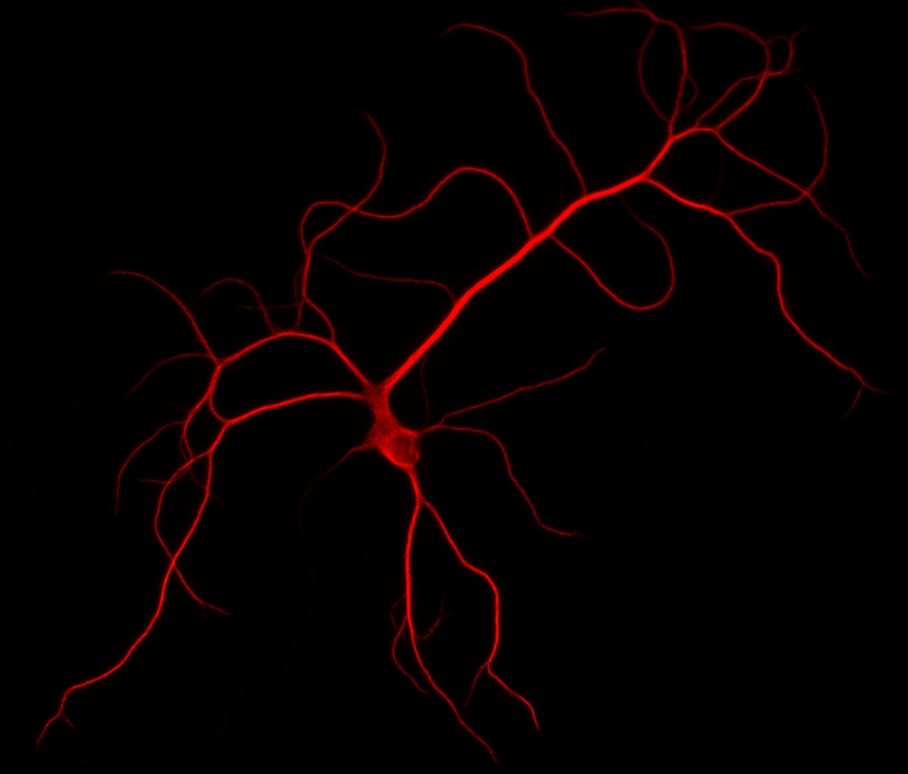
\includegraphics[height=5cm]{images/rat-hippocampal-neuron.jpg}
\vfill
{\tiny Cultured rat hippocampal neuron. Image credit: Ginger Withers. Cell Image Library CIL:36183}
\end{frame}

%--
\begin{frame}
\frametitle{Cable model}

\begin{itemize}
\item Dendrites modelled as idealized electrical cable of variable diameter.
\item Membrane modelled as leaky capacitor with extra current sources.
\end{itemize}
\vfill
\begin{center}
    \begin{tabular}{cc}
	\parbox[c]{0.5\linewidth}{
	    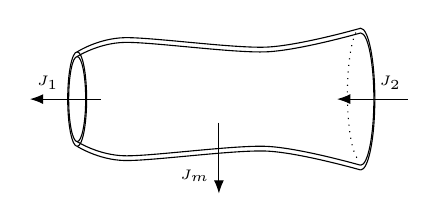
\begin{tikzpicture}[scale=0.6]
		\foreach \r in {-1,1}
		    \foreach \y in {0,-0.1cm}
			\draw[yscale=\r] plot[smooth,yshift=\y] coordinates{(0,1) (1,1.3) (4,1.1) (6,1.5)};
		\draw (0,0) ellipse [x radius=0.2cm, y radius=1cm];
		\draw (0,0) ellipse [x radius=0.18cm, y radius=0.9cm];
		\draw (6,-1.5) arc [start angle=-90, end angle=90, x radius=0.3cm, y radius=1.5cm];
		\draw (6,-1.4) arc [start angle=-90, end angle=90, x radius=0.28cm, y radius=1.4cm];
		\draw[dotted] (6,1.5) arc [start angle=90, end angle=270, x radius=0.28cm, y radius=1.4cm];
		\draw[-Latex] (0.5,0) -- node[above, near end] {\tiny $J_1$} (-1,0);
		\draw[-Latex] (7,0) -- node[above, near start] {\tiny $J_2$} (5.5,0);
		\draw[-Latex] (3,-0.5) -- node[left, near end] {\tiny $J_m$} (3,-2);
	    \end{tikzpicture}
	}
	&
	\parbox[c]{0.3\linewidth}{
	    \small\centering
	    current balance:\\
	    $J_2-J_1 = J_m$
	}
    \end{tabular}
\end{center}
\vfill
\end{frame}

\begin{frame}
\frametitle{Membrane currents}

Mixture of current densities and discrete currents.
\vfill
\begin{tabular}{cc}
    \parbox[c]{0.5\linewidth}{
	\begin{itemize}
	\item Capacitive: $j=c_m \frac{\partial v}{\partial t}$.
	\item Resistive: $j=r_m(v - e^{\rev})$.
	\item Distributed ion channels: $j = g_k(v, t)(v - e_k^{\rev})$.
	\item Synapses at $x_i$: $I = g^{\syn}_i(v - e^{\syn}_i)\delta_{x_i}$.
	\item Current injections at $x_i$: $I = I^{\hbox{\tiny inj}}_i(t)\delta_{x_i}$.
	\end{itemize}
    }
    &
    \parbox[c]{0.5\linewidth}{
        \begin{circuitikz}[american, scale=0.6, every node/.style={scale=0.7}]
            \draw (0,4) -- node[above]{\small intracellular}(8,4);
            \draw (1,4) to[C=$c_m$] (1,0);
            \draw (3,4) to[R=$r_m$] (3,2) to[V<=$e^{\rev}$] (3,0);
            \draw (5,4) to[vR=$g_k^{-1}$] (5,2) to[V=$e_k^{\rev}$] (5,0);
            \draw (7,0) to[I, i_=$I^{\hbox{\tiny inj}}$] (7,4);
            \draw (0,0) -- node[below]{\small extracellular}(8,0);
        \end{circuitikz}
    }
\end{tabular}

\vfill
\end{frame}

%--
\begin{frame}
\frametitle{Cable PDE}
\begin{align*}
\frac{\partial}{\partial x}\left(\sigma\frac{\partial v}{\partial x}\right)
&=
\left(c_m\frac{\partial v}{\partial t} + r_m(v-e^{\rev}) +
\!\!\!\sum_{\text{channels $k$}}\!\!\! g_k(v, t)(v-e_k^{\rev})\right)\cdot\frac{\partial S}{\partial x} \\
&+
\!\!\!\sum_{\text{synapses $k$}}\!\!\! I^{\syn}_k(v, t)\delta_{x_k} +
\!\!\!\sum_{\text{injections $k$}}\!\!\! I^{\hbox{\tiny inj}}_k(t)\delta_{x_k}
\end{align*}

\begin{itemize}
\item $\sigma(x)$ is the axial conductivity, $\propto$ cross-sectional area.
\item $S(x)$ is the surface area as a function of $x$.
\item Discrete current sources are only piece-wise continuous.
\item Ion channel conductivites $g_k(v, t)$ governed by ODEs.
\end{itemize}
\end{frame}

%--
\begin{frame}
\frametitle{Cell state evolution in \nestmc{}}

\begin{itemize}
\item Finite volume discretization in space.
\item Implicit Euler integration up to source discontinuities.
\item Voltage and channel state time evolution split (Lie-Trotter).
\item Channel state ODEs described by DSL (subset of NMODL).
\end{itemize}
\vfill
First order in space and time, but higher order time methods are possible and practical.
\vfill
Typical maximum $dt$ $\sim$ 0.025\ ms.
\vfill
\end{frame}

%--
\begin{frame}
\frametitle{Spiking}

Spikes are an idealized model for action potential propagation along axons to
synapses on other neurons.
\vfill
\begin{itemize}
\item A spike is generated on a neuron when the voltage exceeds a threshold.
\item Spike is transmitted to up to circa. $6\times10^4$ synapses on other neurons,
after a propagation delay $\sim$ 1\ ms.
\item Synapses change their state discontinuously when they receive a spike.
\item Minimum propagation delay allows decoupled, distributed simulation
of neurons.
\end{itemize}
\end{frame}

%--
\begin{frame}
\frametitle{Spike exchange in \nestmc{}}

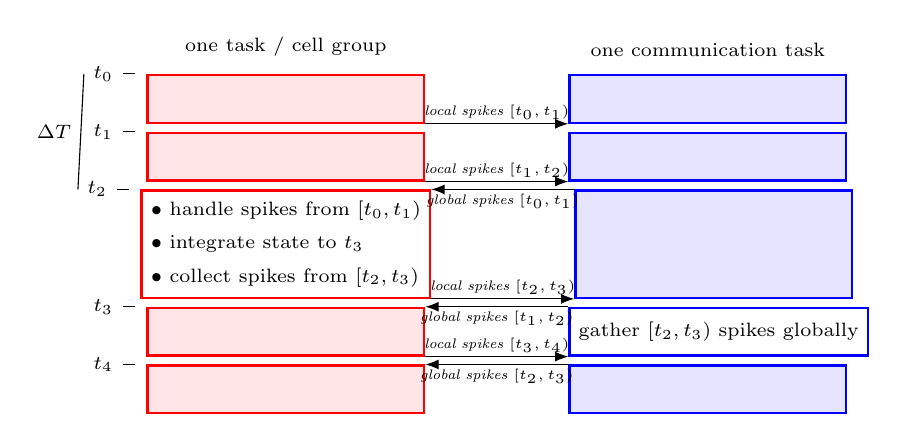
\begin{tikzpicture}
    [procae/.style={rectangle, draw=red, fill=red!10, thick, minimum height=4ex, minimum width=10em},
     procat/.style={rectangle, draw=red, thick, minimum height=4ex, minimum width=10em},
     procbe/.style={rectangle, draw=blue, fill=blue!10, thick, minimum height=4ex, minimum width=10em},
     procbt/.style={rectangle, draw=blue, thick, minimum height=4ex, minimum width=10em},
     tn/.style={minimum width=1em, align=left}]

    \node [procae] (y)  {};
    \node [procbe, right=12ex of y] (z) {};
    \path [-Latex] (y.south east) edge node [above=-2pt] {\tiny\it local spikes $[t_0, t_1)$} (z.south west);
    \node [procae, below=1mm of y] (a)  {};
    \node [procbe, right=12ex of a] (b) {};
    \path [-Latex] (a.south east) edge node [above=-2pt] {\tiny\it local spikes $[t_1, t_2)$} (b.south west);
    \node [procat, below=1mm of a, minimum height=9ex, align=left] (c) {
	\scriptsize $\bullet$ handle spikes from $[t_0, t_1)$\\
	\scriptsize $\bullet$ integrate state to $t_3$\\
	\scriptsize $\bullet$ collect spikes from $[t_2, t_3)$
    };
    \node [procbe, right=12ex of c.south east, anchor=south west, minimum height=9ex] (d) {};
    \path [Latex-] (c.north east) edge node [below=-2pt] {\tiny\it global spikes $[t_0, t_1)$} (d.north west);
    \path [-Latex] (c.south east) edge node [above=-2pt] {\tiny\it local spikes $[t_2, t_3)$} (d.south west);
    \node [procae, below=1mm of c] (e)  {};
    \node [procbt, right=12ex of e] (f) { \scriptsize gather $[t_2,t_3)$ spikes globally };
    \path [Latex-] (e.north east) edge node [below=-2pt] {\tiny\it global spikes $[t_1, t_2)$} (f.north west);
    \path [-Latex] (e.south east) edge node [above=-2pt] {\tiny\it local spikes $[t_3, t_4)$} (f.south west);
    \node [procae, below=1mm of e] (g)  {};
    \node [procbe, right=12ex of g] (h) {};
    \path [Latex-] (g.north east) edge node [below=-2pt] {\tiny\it global spikes $[t_2, t_3)$} (h.north west);

    \draw ([xshift=-1ex] y.north west) -- ++(-1ex, 0) node [tn, left] (p) {\scriptsize $t_0$};
    \draw ([xshift=-1ex] a.north west) -- ++(-1ex, 0) node [tn, left] {\scriptsize $t_1$};
    \draw ([xshift=-1ex] c.north west) -- ++(-1ex, 0) node [tn, left] (q) {\scriptsize $t_2$};
    \draw ([xshift=-1ex] e.north west) -- ++(-1ex, 0) node [tn, left] {\scriptsize $t_3$};
    \draw ([xshift=-1ex] g.north west) -- ++(-1ex, 0) node [tn, left] {\scriptsize $t_4$};

    \draw (p.west) -- node [left] {\scriptsize $\Delta T$} (q.west);

    \node [above=1mm of y.north] {\scriptsize one task / cell group};
    \node [above=1mm of z.north] {\scriptsize one communication task};
\end{tikzpicture}
\vfill
\centering
Overlapping computation and communication.\\
$\Delta T$ is the minimum spike propagation delay.
\end{frame}

%--
\begin{frame}
\frametitle{Work organization --- CPU}

\begin{itemize}
\item One cell is integrated per task.
\item Tasks distributed across thread pool.
\item Cell states typically fit within L3 cache; 
\item Each \emph{mechanism} (ion channel or synapse type) integrated in turn for locality (SoA layout).
\item Implicit Euler step: solve nearly tridiagonal system by Gaussian elimination.
\item Vectorized mechanism code available with Intel compiler.
\end{itemize}
\vfill
\end{frame}

%--
\begin{frame}
\frametitle{Work organization --- GPU}

\begin{itemize}
\item Many (up to circa $10^4$) cells in a group, one group per GPU.
\item Mechanism states are integrated across whole group per mechanism for parallelism.
\item Implicit Euler step: matrix data is interleaved in GPU memory for better memory utilization,
one thread per cell.
\item \emph{Matrix solver still a bottle-neck in models with simple cells.}
\end{itemize}
\vfill
\end{frame}

%--
\begin{frame}
\frametitle{Development}
Current work:
\begin{itemize}
\item Moving more of spike delivery and state inspection to GPU.
\item Generalization of internal cell API to support 'artificial' cells.
\item KNL-specific vectorized kernels.
\item Preparation of realistic benchmark models.
\item Preparation of code for initial release.
\end{itemize}
\vfill
Development on GitHub: \texttt{github.com:eth-cscs/nestmc-proto}
\end{frame}
%
\end{document}
